% !TEX root = 0_main.tex
\chapter{{SkipGate}: Reducing Sequential Overhead}\label{chap:skipgate}
\gls{skipgate} is developed to work with the \acrfull{gc} protocol to reduce the overhead of sequential circuits.
It allows secure evaluation of functions in the form of $o = f(a, b, p)$ where $p$ is the public input known to both parties and $a$ and $b$ are the private inputs.
The goal of \gls{skipgate} is to reduce the circuit of $f(a, b, p)$ into a simpler circuit of $o = f_p(a,b)$ with the same logic for a given public input $p$.
Secure evaluation of $f_p(a,b)$ costs less than that of $f(a, b, p)$ using the conventional \acrshort{gc} protocol where $p$ is treated as a private input.
For doing so, \gls{skipgate} removes communication cost of garbling for a gate when its output can either be computed independently by Alice and Bob or has no effect on the final output.
In other words, \gls{skipgate} reduces the communication between the parties when when less costly local computation can replace it.
The cost reduction is especially significant in a sequential circuit where the control path is public and independent of the private inputs.

In this chapter, first, we introduce the notation used in the \gls{skipgate} algorithm.
Next, a motivational example is provided to present the sequential overhead.
Next, We discuss how gates in a circuit are categorization in \gls{skipgate}.
The pseudo-code of the \gls{skipgate} algorithm is then provided with its complexity analysis and correctness and security proofs.

\section{Notations}\label{sec:skipgate-notation}
In a classic Boolean circuit, each wire $w$ carries a value ($x_w\in\{0, 1\}$), whereas in a garbled circuit, each wire carries a pair of labels ($X_w^{0}$ and $X_w^{1}$) on Alice's side and one label ($X_w \in \{X_w^{0}, X_w^{1}\}$) on Bob's.
If $X_w = X_w^{0}$, the actual Boolean value is 0 and if $X_w = X_w^{1}$, it is 1.
This construction means that the information is shared between two parties.
In our scheme, we combine these notions of Boolean and garbled circuits.
Each wire either carries a Boolean value known to both parties independently (\textit{public} wire), or it carries a (pair of) label(s) (\textit{secret} wire).

\section{Motivational Example}\label{sec:skipgate-motiv}
\fig{fig:mux} illustrates a sequential circuit that has a control path with a 2-to-1 \acrfull{mux} whose inputs come from two sub-circuits f$_0$ and f$_1$ connecting to \acrshort{mux} input 0 and 1 respectively.
At a certain sequential cycle, if the select wire of the \acrshort{mux} ($x$) is public, say equal to 1, both parties know that the gates in the sub-circuit f$_0$ do not need to be garbled/evaluated since they have no effect on the final output.
The gates in the \acrshort{mux} itself act as wires and pass the output of f$_1$ to the \acrshort{mux} output.
Thus, the gates in the control path do not need to be garbled/evaluated in that sequential cycle either.
However, in the conventional \acrshort{gc} protocol where public wire $x$ was teared as a secret value, the entire circuit had to be garbled/evaluated.
In the following subsection, we explain how the \gls{skipgate} algorithm identifies such gates to reduce the garbling cost in circuits with public wires.

\begin{figure}
    \centering
    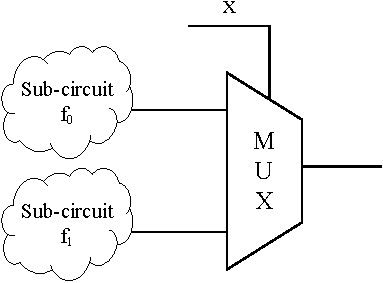
\includegraphics[width = 0.45\textwidth]{mux-crop.pdf}
    \caption{Motivational example: two sub-circuits connecting to a \acrshort{mux} with a public select signal.}
\label{fig:mux}
\end{figure}

It is worth noting that in a sequential garbled circuit presented in \chap{chap:seq}, the Boolean value of a wire can change at every sequential cycle.
A wire may also alter between being secret and public.
The \gls{skipgate} algorithm is executed once for each sequential cycle.
\gls{skipgate}'s decision on each gate (locally computing, garbling/evaluating, or skipping) depends on the status of the gate's inputs (public or secret) on that cycle.
Thus, \gls{skipgate} is fundamentally different compared to offline circuit simplification methods such as the one introduced in~\cite{pinkas2009secure} which remove gates with known constant inputs.
Since we use \gls{tinygarble} to create the circuits, the logic synthesis tool already removed the constant gates in it.

\section{Gate Categories}\label{sec:skipgate-cat}
The \gls{skipgate} algorithm classifies the gates into four categories regarding the parties' knowledge about their inputs:

\begin{enumerate}[label=\roman*]
  \item \textit{Gate with two public inputs.}
    In this case, the output is public.
  \item \textit{Gate with one public input.}
  	Depending on the gate type, the output becomes either public or secret.
  	For example, for an AND gate with 0 at one input, the output becomes 0.
  	This means that if the secret input is not connected to any other gate, the gate generating it can be skipped for garbling/evaluation.
  	If the public input is 1, then the AND gate acts like a wire, and the output wire carries the label of the secret input.
  \item \textit{Gate with secret inputs that have identical (or swapped) labels.}
    This indicates that the two secret inputs have identical (or inverted) Boolean values.
    (In \sect{ssec:skipgate-ident}, we will explain how Bob identifies the swapped case.)
    Depending on the gate type, the output becomes either public or secret.
    For example, the output of an XOR gate with two inverted inputs (either secret or public) is always 1 (public).
  	Similar to Category ii, the gate generating the inputs, if not connected to any other gates, can be skipped for garbling/evaluation.
  \item \textit{Gate with unrelated secret inputs.}
  	The output is always secret.
  	The gate has to be garbled/evaluated conventionally according to the \acrshort{gc} protocol.
    However, if its output does not have any effect on the circuit output, the gate is skipped, i.e., Alice does not send the corresponding garbled table to Bob.
\end{enumerate}

\section{Algorithm}\label{sec:skipgate-alg}

\begin{algorithm}
\caption{\gls{skipgate}, Alice's side.}\label{alg:alice}
\textbf{Inputs:} Sequential \texttt{circuit} of $f(a,b,p)$, Alice's input $a$, public input $p$, number of sequential cycles $cc$.\\
\textbf{Outputs:} $o = f(a,b,p)$.\\
\begin{algorithmic}[1]
\STATE{\bf{SkipGate\_alice\ (circuit, a, p, cc)}:}
\STATE{($X^0_a,X^1_a,X^0_b,X^1_a$) = generate\_random\_labels()}
\STATE{send\_alice\_labels($a, X^0_a, X^1_a$)}
\STATE{send\_bob\_labels($X^0_b, X^1_b$) \textit{ // through \acrshort{ot}}}
\STATE{circuit.set\_private\_input($X^0_a,X^1_a,X^0_b,X^1_a$)}
\STATE{circuit.set\_public\_input($p$)}
\FOR{cid in [$0 ... cc-1$]}
  \STATE{circuit.initial\_label\_fanout()}
  \STATE{circuit.phase1()}
  \STATE{garbled\_tables = circuit.phase2\_alice()}
  \STATE{send\_garbled\_tables(garbled\_tables)}
  \STATE{circuit.transfer\_flip\_flops\_labels()}
\ENDFOR
\STATE{($X^0_c,X^1_c$) = circuit.get\_output\_label()}
\STATE{$X_c$ = receive\_bob\_output\_label()}
\STATE{$o$=get\_output\_value($X^0_o,X^1_o,X_o$)}
\end{algorithmic}
\end{algorithm}

\begin{algorithm}
\caption{\gls{skipgate}, Bob's side.}\label{alg:bob}
\textbf{Inputs:} Sequential \texttt{circuit} of $f(a,b,p)$, Bob's input $b$, public input $p$, number of sequential cycles $cc$.\\
\begin{algorithmic}[1]
\STATE{\bf{SkipGate\_bob(circuit, b, p, cc)}:}
\STATE{$X_a$ = receive\_alice\_labels()}
\STATE{$X_b$ = receive\_bob\_labels($b$) \textit{//through \acrshort{ot}}}
\STATE{circuit.set\_private\_input($X_a,X_b$)}
\STATE{circuit.set\_public\_input($p$)}
\FOR{cid in [$0 ... cc-1$]}
  \STATE{circuit.initial\_label\_fanout()}
  \STATE{circuit.phase1()}
  \STATE{garbled\_tables = receive\_garbled\_tables()}
  \STATE{circuit.phase2\_bob(garbled\_tables)}
  \STATE{circuit.transfer\_flip\_flops\_labels()}
\ENDFOR
\STATE{$X_c$ = circuit.get\_output\_label()}
\STATE{send\_output\_label($X_o$)}
\end{algorithmic}
\end{algorithm}

\alg{alg:alice} and \alg{alg:bob} show the \gls{skipgate} algorithm for Alice and Bob sides respectively.
Lines 2-5 of \alg{alg:alice} and Lines 2-4 of \alg{alg:bob} are similar to the \acrshort{gc} protocol label generation and transfer for both sides.
The \gls{skipgate} algorithm has two main phases:
In Phase 1, the parties compute the outputs of the gates with public input (Categories i-ii).
In Phase 2, they garble/evaluate the gates with private inputs (Categories iii-iv).
For each round of sequential cycle, Alice executes Phase 1 and 2 of \gls{skipgate} and sends the generated garbled tables to Bob.
Bob receives the tables and executes two phases to evaluate the gates.
In Line 12 of \alg{alg:alice} and Line 11 of \alg{alg:bob}, the labels associated with the input of flip-flops are transferred to their output for the next cycles as required by sequential \acrshort{gc} protocol (see \sect{sec:seq-seq}).
Similar to conventional \acrshort{gc}, in the end, Alice learns pairs of labels for each output wire and Bob has one of the pairs; they share this information to learn the output $o$.
For example, in the case where Alice intends to learn the final output, she receives Bob's output label and together with her input labels finds the real output value (Line 15-16 of \alg{alg:alice} and Line 14 of \alg{alg:bob}).

In \gls{skipgate}, an integer called \texttt{label\_fanout} is associated with each gate and indicates the number of times the gate's output label is used (either as a circuit's output or as an input to other gates).
At the beginning of each cycle (Line 8 of \alg{alg:alice} and \alg{alg:bob}), the parties set the \texttt{label\_fanout} to the gate fanout in the circuit\footnote{\textit{Fanout} of a gate, borrowed from hardware design, is the number of subsequent gates (and circuit outputs) dependent on the gate’s output.}.
A gate's \texttt{label\_fanout} may decrease if its output label is not needed anymore, e.g., a gate whose output is connected an AND gate with 0 at the other input (Category ii).
If \texttt{label\_fanout} reaches 0, it means that gate's output label does not have any effect on the final output.
The gates with \texttt{label\_fanout}=0 are subsequently designated for skipping, which in turn decreases the \texttt{label\_fanout} of their input gates recursively.
Finally, the gates in Category iv that the parties have not marked for skipping are garbled/evaluated.

\begin{algorithm}
\caption{Phase 1 in \gls{skipgate} for both Alice and Bob sides.}\label{alg:phase1}
\begin{algorithmic}[1]
\STATE{\bf{circuit.phase1()}:}
\FOR{g in circuit}
	\IF{g.i0 is public and g.i1 is public \textit{//Category i}}
		\STATE{g.o = public\_calculate(g.type, g.i0, g.i1)}
		\STATE{g.label\_fanout $= 0$}
	\ELSIF{g.i0 is public or g.i1 is public \textit{//Category ii}}
		\STATE{g.o = g.half\_public\_calculate(g.type, g.i0, g.i1)}
		\IF{g.o is public}
			\STATE{g.label\_fanout $= 1$ \textit{//will become zero in recursive\_reduction()}}
			\STATE{circuit.recursive\_reduction(g)}
		\ENDIF
	\ENDIF
\ENDFOR
\end{algorithmic}
\end{algorithm}

\alg{alg:phase1} illustrates Phase 1 of \gls{skipgate} in which Alice and Bob find and compute the gates that belong to Categories i-ii.
They set the \texttt{label\_fanout}s of the gates in Category i to zero.
For gates in Category ii, if the output becomes public, \gls{skipgate} decreases the \texttt{label\_fanout} of the secret input's originating gates recursively by invoking \texttt{recursive\_reduction} (\alg{alg:skipgate_reduction}).
\fig{fig:phaseOneExample} shows four different examples in Phase 1.

Bob does not receive any information from Alice about the gates in Category i-ii because he can locally evaluate Phase 1 just like Alice.
An alternative approach is that Alice sends the result of Phase 1 to Bob.
This method has two main disadvantageous:
First, it makes the protocol complicated if one wants to enhance the security of the protocol to be secure against malicious adversaries.
Second, it increases the communication overhead which is the bottleneck of the \acrshort{gc} protocol.

\begin{figure}
    \centering
    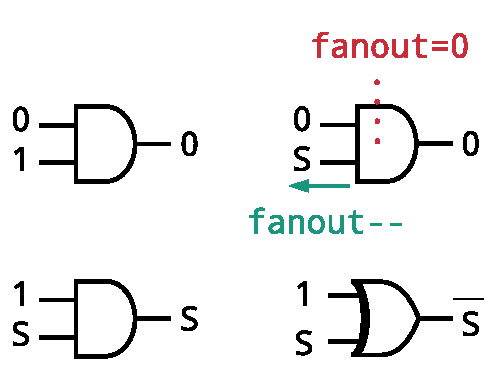
\includegraphics[width=0.40\textwidth]{phaseOneExample-crop.pdf}
    \caption{Four examples of replacing gates in Phase 1 by zero, one, wire, or inverter.
    \texttt{label\_fanout} is decreased for the unnecessary gate.
    The top-left example is in Category i and the rest are in Category ii.}
    \label{fig:phaseOneExample}
\end{figure}

\begin{algorithm}
\caption{Phase 2 in \gls{skipgate}, Alice's side.}\label{alg:phase2_alice}
\textbf{Output}: \texttt{garbled\_tables} queue.\\
\begin{algorithmic}[1]
\STATE{\bf{circuit.phase2\_alice()}:}
\FOR{g in circuit where g.label\_fanout $> 0$}
	\IF{(g.i0.label is equal g.i1.label or\\
		g.i0.label is inverted g.i1.label) \textit{//Category iii}}
		\STATE{g.o = related\_secret\_calculate(g.type, g.i0, g.i1)}
		\IF{g.o is public}
			\STATE{g.label\_fanout $= 1$ \textit{//will become zero in recursive\_reduction()}}
			\STATE{circuit.recursive\_reduction(g)}
		\ENDIF
	\ELSE \STATE{\textit{//Category iv}}
    \STATE{(g.o, g.table) = garble(g.type, g.i0, g.i1) \textit{//table=null for XOR}}
    \IF{g is non-XOR}
      \STATE{garbled\_tables.enqueue(g.id, g.table)}
    \ENDIF
	\ENDIF
\ENDFOR
\STATE{garbled\_tables.filter(t : circuit[t.id].label\_fanout $> 0$)}
\end{algorithmic}
\end{algorithm}

\alg{alg:phase2_alice} shows the Phase 2 of \gls{skipgate} for Alice's side in which she performs the same task for Category iii.
She then generates garbled tables for gates with non-zero \texttt{label\_fanout} in Category iv.
\fig{fig:phaseTwoExample} shows four different examples in this phase.
By the end of Phase 2, due to the recursive nature of the fanout reduction, \texttt{label\_fanout} of some gates that have already been garbled may become 0.
In Line 17 of \alg{alg:phase2_alice}, Alice filters the garbled tables that have non-zero \texttt{label\_fanout} to be sent to Bob.

\begin{figure}
    \centering
    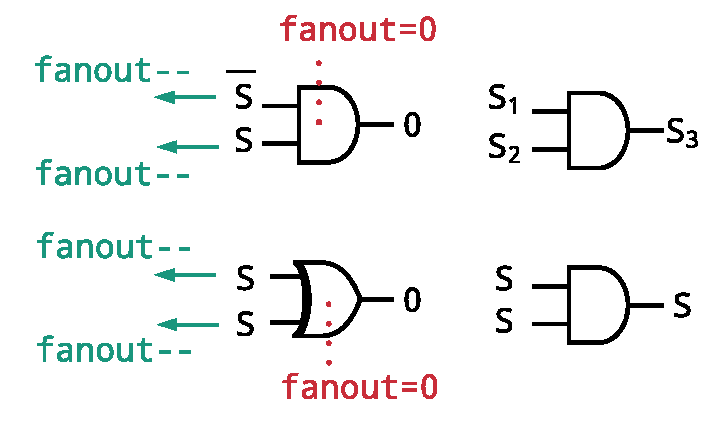
\includegraphics[width = 0.50\textwidth]{phaseTwoExample-crop.pdf}
    \caption{Four examples of replacing and computing gates in Phase 2.
    		 \texttt{label\_fanout} is decreased for the unnecessary gates.
         The top-right example is in Category iv, and the rest are in Category iii.}
    \label{fig:phaseTwoExample}
\end{figure}

\begin{algorithm}
\caption{Phase 2 in \gls{skipgate}, Bob's side.}\label{alg:phase2_bob}
\textbf{Input}: \texttt{garbled\_tables} queue.\\
\begin{algorithmic}[1]
\STATE{\bf{circuit.phase2\_bob(garbled\_tables)}:}
\FOR{g in circuit where g.label\_fanout $> 0$}
	\IF{(g.i0.label is equal g.i1.label or\\
		g.i0.label is inverted g.i1.label) \textit{//Category iii}}
		\STATE{g.o = related\_secret\_calculate(g.type, g.i0, g.i1)}
		\IF{g.o is public}
			\STATE{g.label\_fanout $= 1$ \textit{//will become zero in recursive\_reduction()}}
			\STATE{circuit.recursive\_reduction(g)}
		\ENDIF
	\ELSE \STATE{\textit{//Category iv}}
    \IF{g is XOR}
     \STATE{g.o = g.eval\_XOR(g.i0, g.i1)}
    \ELSIF{g.id is garbled\_tables.top().id}
      \STATE{gt = garbled\_tables.dequeue().table}
      \STATE{g.o = g.eval(g.type, g.type, g.i0, g.i1, gt)}
    \ELSE
      \STATE{g.o = next\_unique\_label() \textit{//generate a unique label.}}
    \ENDIF
	\ENDIF
\ENDFOR
\end{algorithmic}
\end{algorithm}

\alg{alg:phase2_bob} shows the Phase 2 for Bob's side.
Bob evaluates the gates that belong to Category iii and iv.
In Line 17 of \alg{alg:phase2_bob}, Bob generates and assigns new unique labels (\texttt{next\_unique\_label}) for gates that were filtered by Alice.
Bob knows that the \texttt{label\_fanout} of these gates will eventually become 0.
Therefore, he produces new labels for them only to keep track of these secret variables that are used to compute the output of the gates in Category iii.
Bob can generate these labels randomly or use a monotonic counter that increases by one for each newly generated label.
To distinguish valid \acrshort{gc} labels from his generated labels, he keeps a single bit flag along with each label that indicates he generated the label and it is not valid for \acrshort{gc} evaluation.

\begin{algorithm}
\caption{Recursive Fanout Reduction of \gls{skipgate}.}\label{alg:skipgate_reduction}
\textbf{Inputs:} Gate \texttt{g} (where the reduction starts).\\
\begin{algorithmic}[1]
\STATE{\bf{circuit.recursive\_reduction(g)}:}
\IF{g.label\_fanout is  0}
	\STATE{return}
\ENDIF
\STATE{g.label\_fanout = g.label\_fanout - 1}
\IF{g.label\_fanout is  0}
	\IF{g.i0 is secret}
		\STATE{circuit.recursive\_reduction(circuit[g.i0])}
	\ENDIF
	\IF{g.i1 is secret}
		\STATE{circuit.recursive\_reduction(circuit[g.i1])}
	\ENDIF
\ENDIF
\end{algorithmic}
\end{algorithm}


\alg{alg:skipgate_reduction} illustrates the pseudo-code for the recursive fanout reduction.
It receives the circuit and a gate of the circuit.
It first decreases the \texttt{label\_fanout} of the given gate.
If the \texttt{label\_fanout} becomes 0, it recursively calls itself with the gates that generate the secret input(s).
\fig{fig:phaseOneRecursive} illustrates this process on a sample circuit.

\begin{figure}
    \centering
    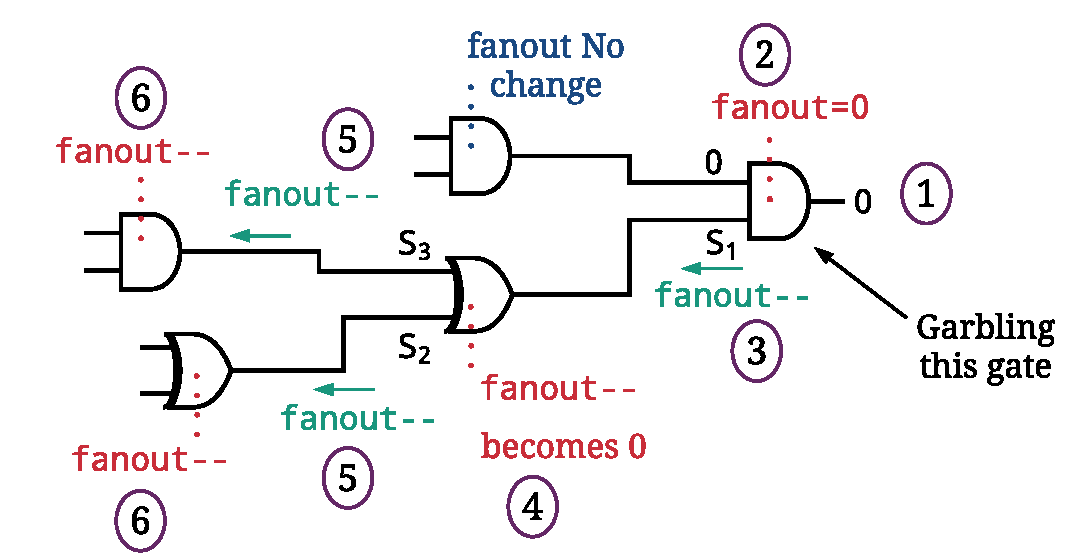
\includegraphics[width=0.8\textwidth]{phaseOneRecursiveExample-crop.pdf}
    \caption{Recursive reduction of \texttt{label\_fanout} to skip unnecessary gates in Phase 1.}
    \label{fig:phaseOneRecursive}
\end{figure}

\subsection{Identification of Identical and Inverted Labels}\label{ssec:skipgate-ident}
According to the \acrshort{gc} protocol, Bob receives only one label $X_w$ for each secret wire $w$.
Due to Free XOR~\cite{kolesnikov2008improved}, he does not need to do anything with a label when it passes a NOT gate because Alice will flip the labels associated with the Boolean value.
Thus, he cannot tell apart an identical and inverted secret values just by storing labels.
However, it is still possible for Bob to keep track of the flips by storing one bit along with the label.
After evaluating a NOT gate, he simply flips the bit.
The extra bit helps him to differentiate between identical and inverted secret values which is crucial for Phase 2.

\fig{fig:mux_annotated} illustrates the effect of \gls{skipgate} on the example in \fig{fig:mux}.
The gates in the sub-circuit f$_0$ will all be skipped for garbling because their \texttt{label\_fanout} will be zero.
The gates in the \acrshort{mux} also will be bypassed since they belong to Groups (i-iii).

\begin{figure}
    \centering
    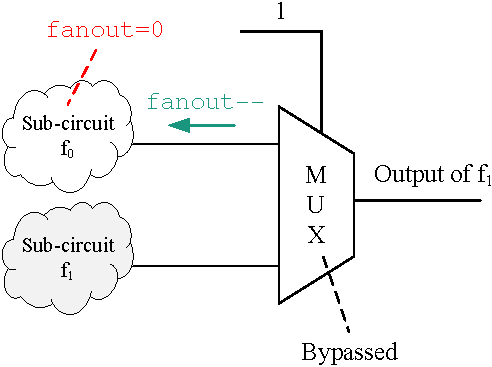
\includegraphics[width = 0.5\textwidth]{mux_annotated-crop.pdf}
    \caption{\gls{skipgate} macro effect on the example in \fig{fig:mux}.
    		 Only sub-circuit f$_1$ is garbled/evaluated.}
\label{fig:mux_annotated}
\end{figure}

\section{Computational Complexity}\label{sec:skipgate-complex}
The \gls{skipgate} algorithm decreases the communication cost of \acrshort{gc}, at the expense of increasing the local computations.
The conventional \acrshort{gc} protocol has a linear computational complexity in terms of the number of gates in the circuit for each sequential cycle.
We show that, despite its recursive appearance, the \gls{skipgate} algorithm does not increase the computation complexity of the \acrshort{gc} protocol.
All parts of the \gls{skipgate} algorithm, except \textit{recursive\_reduction} procedure (\alg{alg:skipgate_reduction}), is executed once per gate, thus they incur a complexity similar to the classic \acrshort{gc} protocol.
The only possible source of complexity increase is \textit{recursive\_reduction} function whose number of invocations depends on the underlying circuit and whether input wires are secret or public.
To find the complexity of \gls{skipgate}, we compute an upper bound on number of invocations of \textit{recursive\_reduction} function.

The termination condition in \textit{recursive\_reduction} is the fanout reaching zero (Lines 2 and 6 of \alg{alg:skipgate_reduction}).
Thus, the worst case scenario is when the function reduces the fanout of all the gates to zero.
In this case, the number of execution of the fanout decrement (Line 5) should be at most the sum of all the initialized fanouts.
The parties initialize \textit{label\_fanout} the gate fanout in the circuit.
The upper bound on the sum of fanouts of all the gates in the circuit is $$F = \sum_{i=1}^{n} g[i].fanout \le 2n - m + q,$$ where $n$ is the number of gates, $q$ is the number of circuit output, and $m$ is the number of circuit inputs.
Each gate has two inputs and each input creates a fanout in previous gates unless it is a circuit input.
Also, each output wire incurs the fanout of one.
Both $q$ and $m$ are typically less than or at most in the order of $n$.
Thus, $F$ and subsequently the number of invocation of \texttt{recursive\_reduction} function are $\BigO{n}$.
This linear complexity shows that \gls{skipgate} does not increase the overall computational complexity of the \acrshort{gc} protocol.

\section{Correctness Proof}\label{sec:skipgate-correct}
Given the correctness of Yao's \acrshort{gc} protocol, we have to show that \acrshort{gc} protocol with \gls{skipgate} is also correct.
\gls{skipgate} does not alter the topology of the circuit.
Thus, the dependencies of the values remain the same.
Therefore, if we can prove that the operation of \gls{skipgate} on a single gate is correct, the entire algorithm is proved to be logically correct.

The operations for gates in Category i are based on the Boolean operation of the gates and are clearly correct.
For gates in Categories ii-iii, we consider the secret input as an unknown variable.
The parties either pass the secret label to the gate's output, or they set the output to a public value.
Since they perform this operation based on the Boolean logic of the pertinent gate, the output remains logically correct.
Gates in Category iv with non-zero \textit{label\_fanout} are garbled/evaluated according to the \acrshort{gc} protocol.
For the rest of the gates in Category iv, \textit{label\_fanout}=0 indicates that their secret output does not have any effect on the final output of the circuit.
Therefore, they can be safely skipped.
As such, we conclude that the algorithm with \acrshort{gc} protocol results in a logically correct output.

\section{Security Proof}\label{sec:skipgate-security}
The \acrshort{gc} protocol is proved to be secure under honest-but-curious adversary model for any two-input Boolean function $f(a, b)$ where $a$ and $b$ are private inputs from Alice and Bob respectively \cite{lindell2009proof, bellare2013efficient}.
In this thesis, we extend the function to the form of $f(a, b, p)$ to include a public input $p$ that is known to both parties.
The \gls{skipgate} algorithm reduces the Boolean circuit of $f(a, b, p)$ to a two-input circuit of $f_p(a, b)$ where, for a given $p$, $f_p(a, b) = f(a, b, p)$ for any $a$ and $b$.
$f_p(a, b)$ consists of the gates in Category iv with non-zero \textit{label\_fanout} evaluated by the \acrshort{gc} protocol.
The process of skipping gates from $f(a, b, p)$ only utilizes the public input $p$ which is already known to both parties.
In the process, the private values are treated as unknown Boolean variables.
In other words, Alice and Bob do not access their inputs in the \gls{skipgate} algorithm for reducing $f(a,b,p)$ to $f_p(a, b)$.
Thus, the \gls{skipgate} algorithm reveals no information about the private inputs $a$ and $b$.
The garbling/evaluation of the two-input Boolean function of $f_p(a,b)$ is passed to the original \acrshort{gc} protocol.
Therefore, the security proof of the \acrshort{gc} protocol still holds for \gls{skipgate}.
